% !TEX TS-program = pdflatex
% !TEX encoding = UTF-8 Unicode

\documentclass[11pt]{article}
\usepackage[utf8]{inputenc} 
\usepackage[parfill]{parskip}
\usepackage[T1]{fontenc} 

\usepackage{fixltx2e}
\usepackage{calc}
\usepackage[export]{adjustbox} % also loads graphicx
\usepackage{makeidx}
\usepackage{multicol}
\usepackage{multirow}
\PassOptionsToPackage{warn}{textcomp}
\usepackage{textcomp}
\usepackage[nointegrals]{wasysym}
\usepackage[table]{xcolor}

\usepackage{csvsimple}

% Font selection
\usepackage[T1]{fontenc}
\usepackage[scaled=.90]{helvet}
\usepackage{courier}
\usepackage{amssymb}
\usepackage{sectsty}

%%% PAGE DIMENSIONS
\usepackage{geometry} % to change the page dimensions
\geometry{a4paper} % or letterpaper (US) or a5paper or....
\geometry{margin=1in} % for example, change the margins to 2 inches all round

\usepackage{graphicx} % support the \includegraphics command and options
\usepackage[parfill]{parskip} % Activate to begin paragraphs with an empty line rather than an indent

%%% PACKAGES
\usepackage{booktabs} % for much better looking tables
\usepackage{array} % for better arrays (eg matrices) in maths
\usepackage{paralist} % very flexible & customisable lists (eg. enumerate/itemize, etc.)
\usepackage{verbatim} % adds environment for commenting out blocks of text & for better verbatim
\usepackage{subfig} % make it possible to include more than one captioned figure/table in a single float
% These packages are all incorporated in the memoir class to one degree or another...
\usepackage{graphicx} 
\graphicspath{ {../analysis/} }

\usepackage{ifpdf}
\ifpdf
\usepackage[pdftex,pagebackref=true]{hyperref}
\else
\usepackage[ps2pdf,pagebackref=true]{hyperref}
\fi
\hypersetup{%
	colorlinks=true,%
	linkcolor=blue,%
	citecolor=blue,%
	unicode%
}


%%% HEADERS & FOOTERS
\usepackage{fancyhdr} % This should be set AFTER setting up the page geometry
\pagestyle{fancy} % options: empty , plain , fancy
\renewcommand{\headrulewidth}{0pt} % customise the layout...
\lhead{}\chead{}\rhead{}
\lfoot{}\cfoot{\thepage}\rfoot{}
%%% END Article customizations

%%% The "real" document content comes below...

\title{PSZT - Uczenie Maszynowe}
\author{Stawczyk Przemysław 293153, Piotr Zmyślony 268833}
\date{} % Activate to display a given date or no date (if empty),
% otherwise the current date is printed 

\begin{document}
	\maketitle
	\setcounter{secnumdepth}{3}
	\setcounter{tocdepth}{3}
	\tableofcontents
	\clearpage
\section{Opis zagadnienia}
\subsection{Treść zadania}
Przedstawić wyniki analizy zbioru \textsl{Bankruptcy}, opisać procedurę eksperymentalną uczenia maszynowego z wykorzystaniem algorytmów \textsl{random forest} i \textsl{k-najbliższych sąsiadów} oraz opisać wyniki strojenia parametrów powyższych algorytmów.
\subsection{Narzędzia}
Skrypty oraz algorytm zostały zaimplementowane w Pythonie 3. Wykorzystano biblioteki: \textsl{imblearn.over\_sampling.SMOTE, sklearn, numpy, matplotlib, scipy.io, impyute}.
\section{Opis preprocesingu i modelowania}
\subsection{Opis danych wejściowych}
Jako dane wejściowe posiadamy 5 plików \textsl{.arff}, z których każdy zawiera ekonomiczne wskaźniki z systemu EMIS na temat polskich firm i ich klasyfikację względem tego, czy firmy zbankrutowały po \textsl{n} latach od roku, w którym zostały zebrane dane. Liczba \textsl{n} lat jest różna dla każdego z plików, od 1 do 5, a każda firma opisana jest przez 64 atrybuty, od \textsl{X1} do \textsl{X64}.
\subsection{Analiza zbioru danych}
\subsubsection{Brakujące dane}
Zaczęliśmy od analizy brakujących danych w wierszach. Jak widać w poniższych wynikach w większości zbiorów około połowa wierszy ma brakujące pola.
\begin{center}
\begin{tabular}{|c|m{0.7in}|m{0.7in}|m{0.7in}|m{0.7in}|m{0.7in}|}
	\hline
	& \textit{1 rok} & \textit{2 lata} & \textit{3 lata} & \textit{4 lata} & \textit{5 lat} \\ \hline
	\textit{długość} & 7027 & 10173 & 10503 & 9792 & 5910 \\ \hline
	\textit{pełne wiersze} & 3194 & 4088 & 4885 & 4769 & 3031 \\ \hline
	\textit{wiersze wybrakowane} & 3833 & 6085 & 5618 & 5023 & 2879 \\ \hline
\end{tabular}
\end{center}
Następnie przeprowadziliśmy analizę rozkładu brakujących danych w kolumnach i wierszach korzystając z biblioteki pythona \textit{missingno} [fig 1-5]\\

\begin{figure}[h]
\caption{1 rok}
	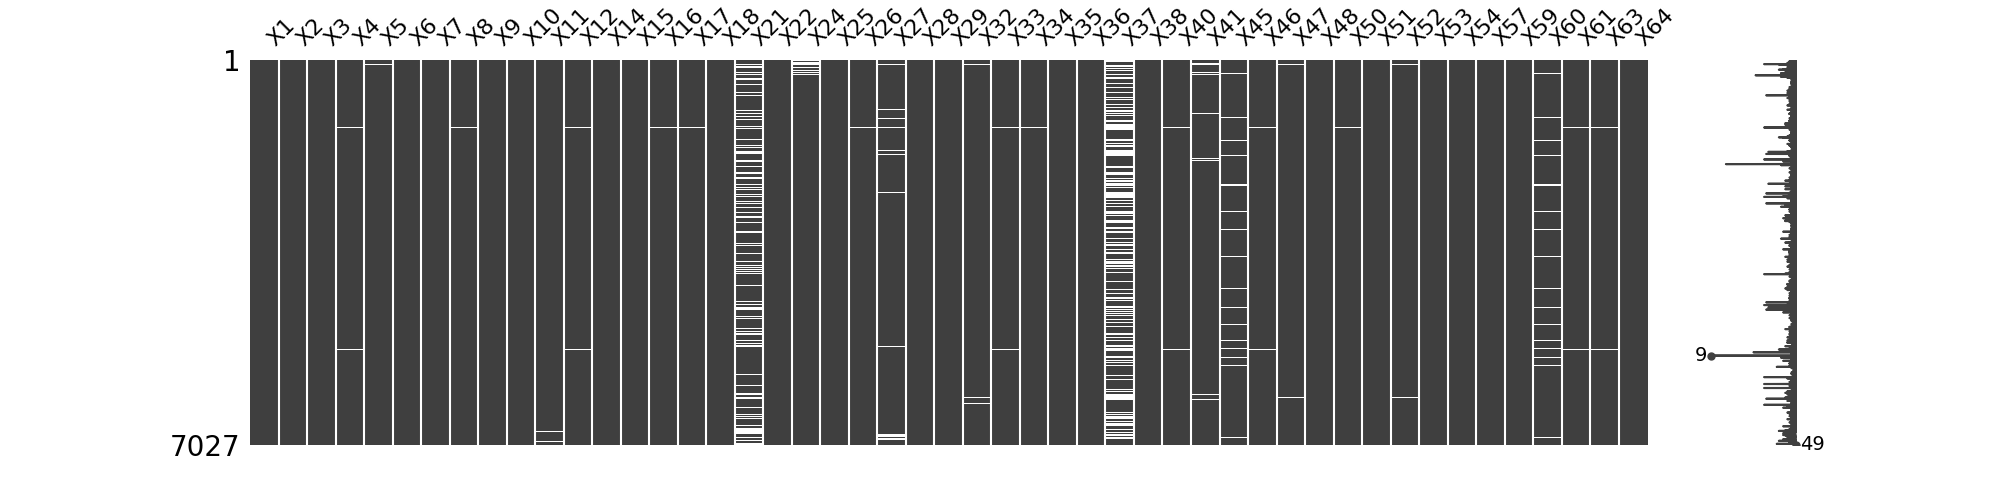
\includegraphics[width=\textwidth]{year_1}
\end{figure}
\begin{figure}[p]
\caption{2 lata}
	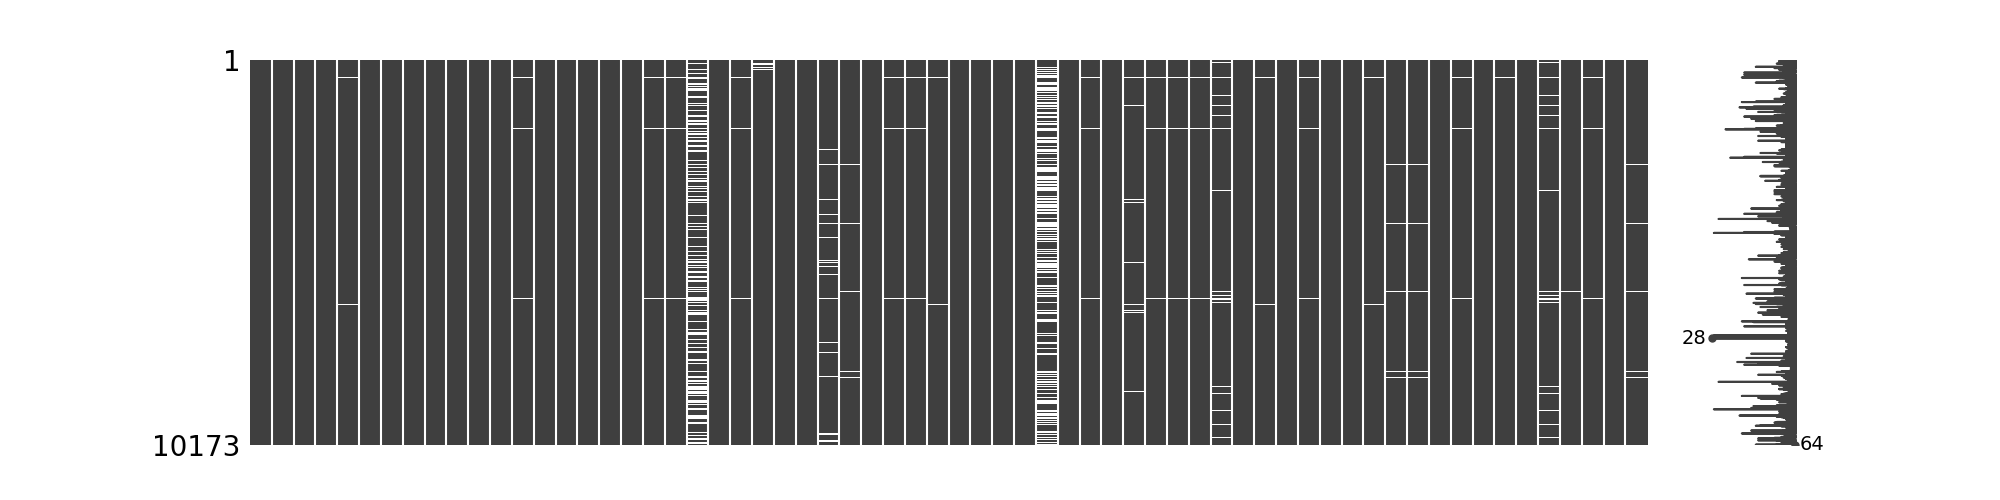
\includegraphics[width=\textwidth]{year_2}
\caption{3 lata}
	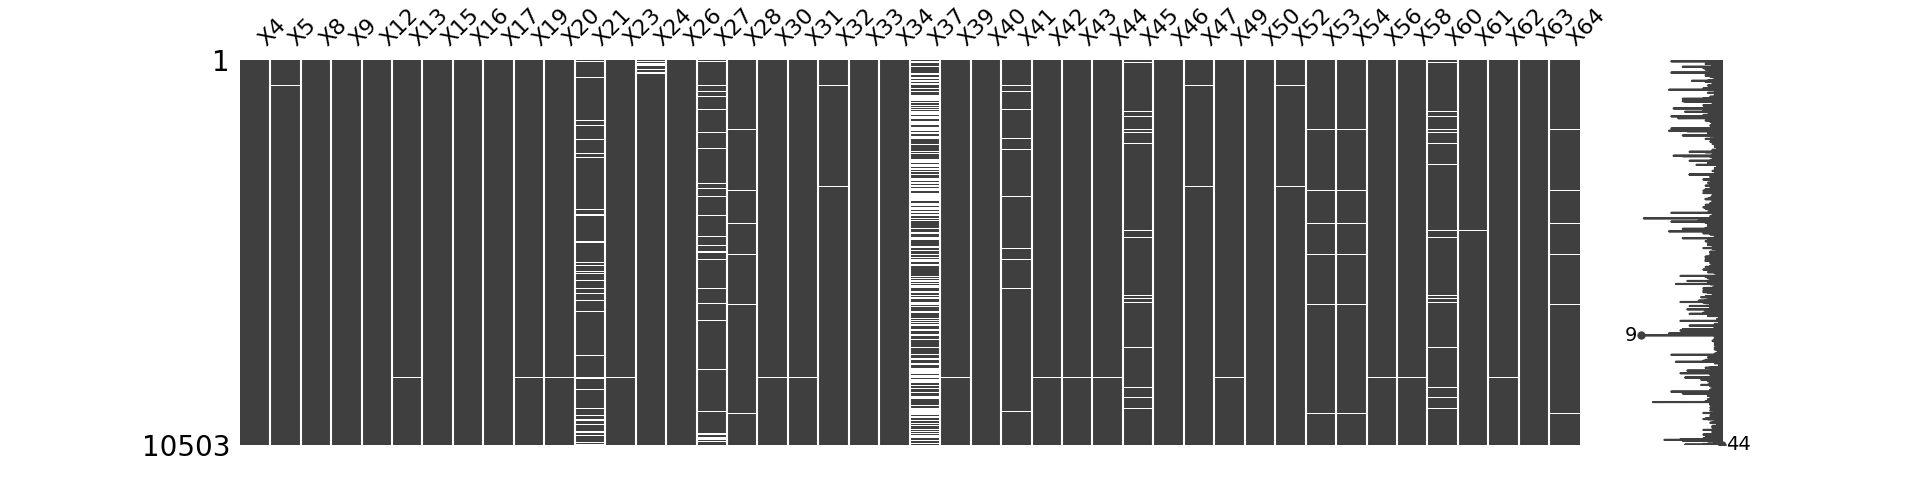
\includegraphics[width=\textwidth]{year_3}
\caption{4 lata}
	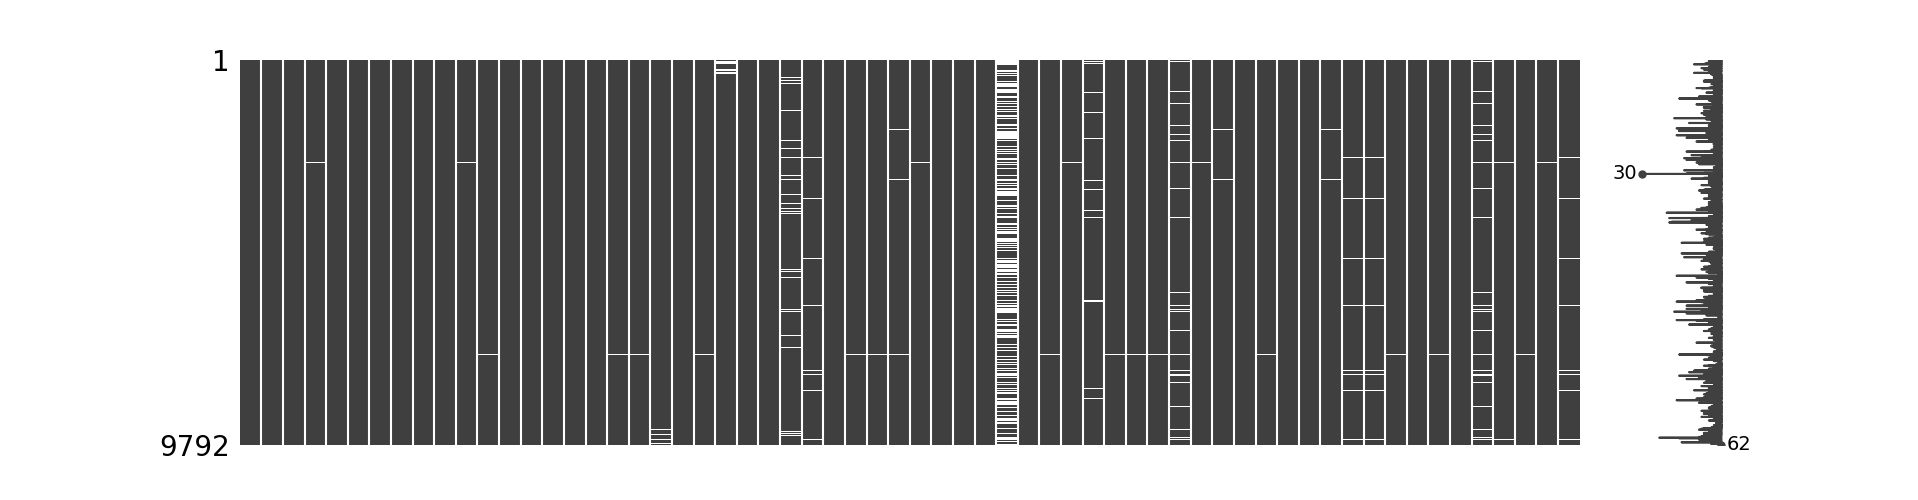
\includegraphics[width=\textwidth]{year_4}
\caption{5 lat}
	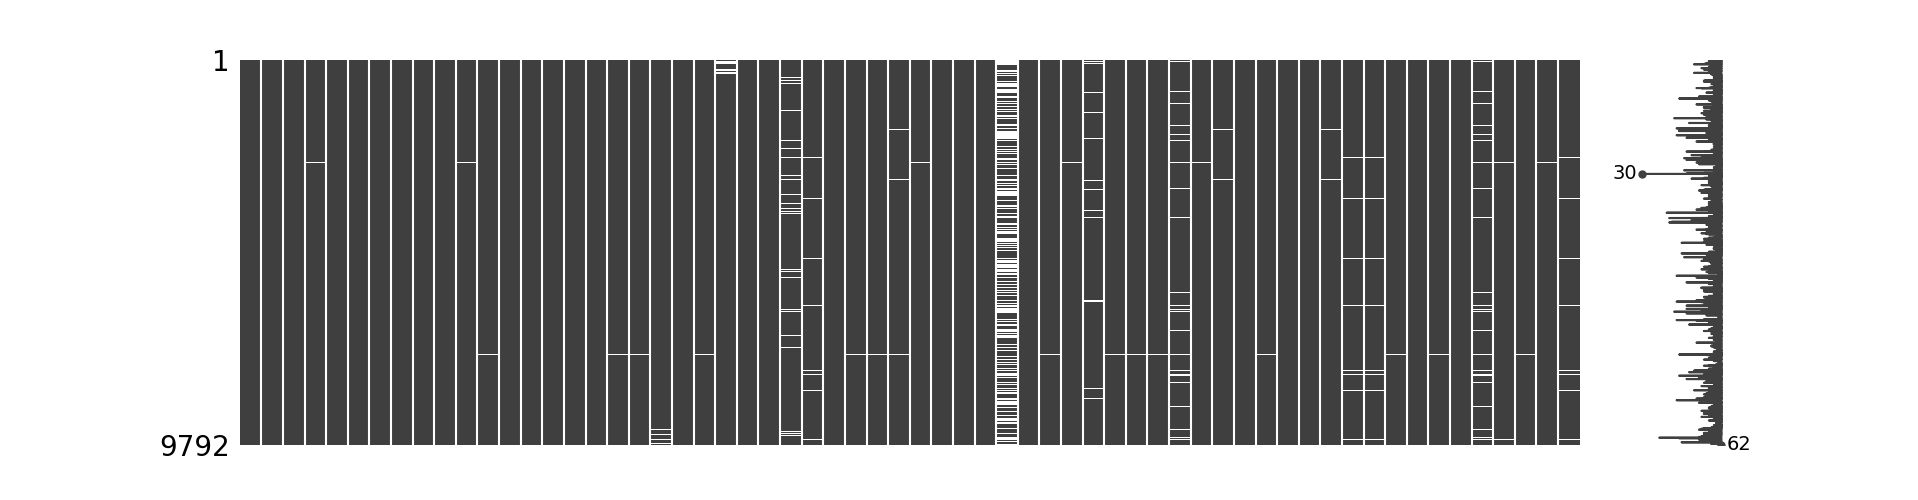
\includegraphics[width=\textwidth]{year_5}
\end{figure}

Jak widać większość brakujących danych jest w kolumnie \textit{X37}. Kolumna \textit{X21} ma brakujące w niektórych ale nie wszystkich latach.\\
Trudno nam było ocenić jaki charakter mają braki w tych danych, czy są skorelowane w wartościami w innych kolumnach czy zupełnie losowe. Wierszy z brakującymi danymi jest około połowy lub więcej. Aby nie odrzucać tak dużej liczby krotek zdecydowaliśmy się interpolować brakujące dane.\\
W tym celu wybraliśmy 4 metody:
\begin{enumerate}
	\item Wstawianie średniej w danej kolumnie \textit{(Jako punkt odniesienia)}
	\item K najbliższych krotek
	\item Spodziewanej Maksymalizacji \textit{(Expected Maximalisation)}
	\item Algorytm MICE
\end{enumerate}
\subsubsection{Zbalansowanie danych}
Dokonaliśmy analizy ile z poszczególnych rekordów należy do klas klasyfikacyjnych
\begin{center}
	\begin{tabular}{|c|m{0.7in}|m{0.7in}|m{0.7in}|m{0.7in}|m{0.7in}|}
		\hline
		\textit{Czy zbankrutowano:}& \textit{rok 1} & \textit{rok 2} & \textit{rok 3} & \textit{rok 4} & \textit{rok 5} \\ \hline
		\textit{Nie} & 6756 & 9773 & 10008 & 9277 & 5500 \\ \hline
		\textit{Tak} & 271 & 400 & 495 & 515 & 410 \\ \hline \hline
		\textit{procent większości} & 3.857 \% & 3.932 \% & 4.713 \% & 5.259 \% & 6.937 \% \\ \hline
	\end{tabular}
\end{center}
Dane w zbiorach są mocno niezbalansowane dlatego zdecydowaliśmy się na interpolację korzystając z metody \textit{SMOTE (Synthetic Minority Over Sampling Technique)}
\subsection{Przepływ Danych}
Po powyższej analizie zdecydowaliśmy o następującym przepływie oryginalnych danych do konstrukcji modeli.\\
Walidacji modeli planujemy dokonać korzystając K-krotnej walidacji krzyżowej.
\subsubsection{Wizualizacja Przepływu Danych}
\begin{figure}[h]
	\caption{Przepływ Danych}
	\begin{center}
		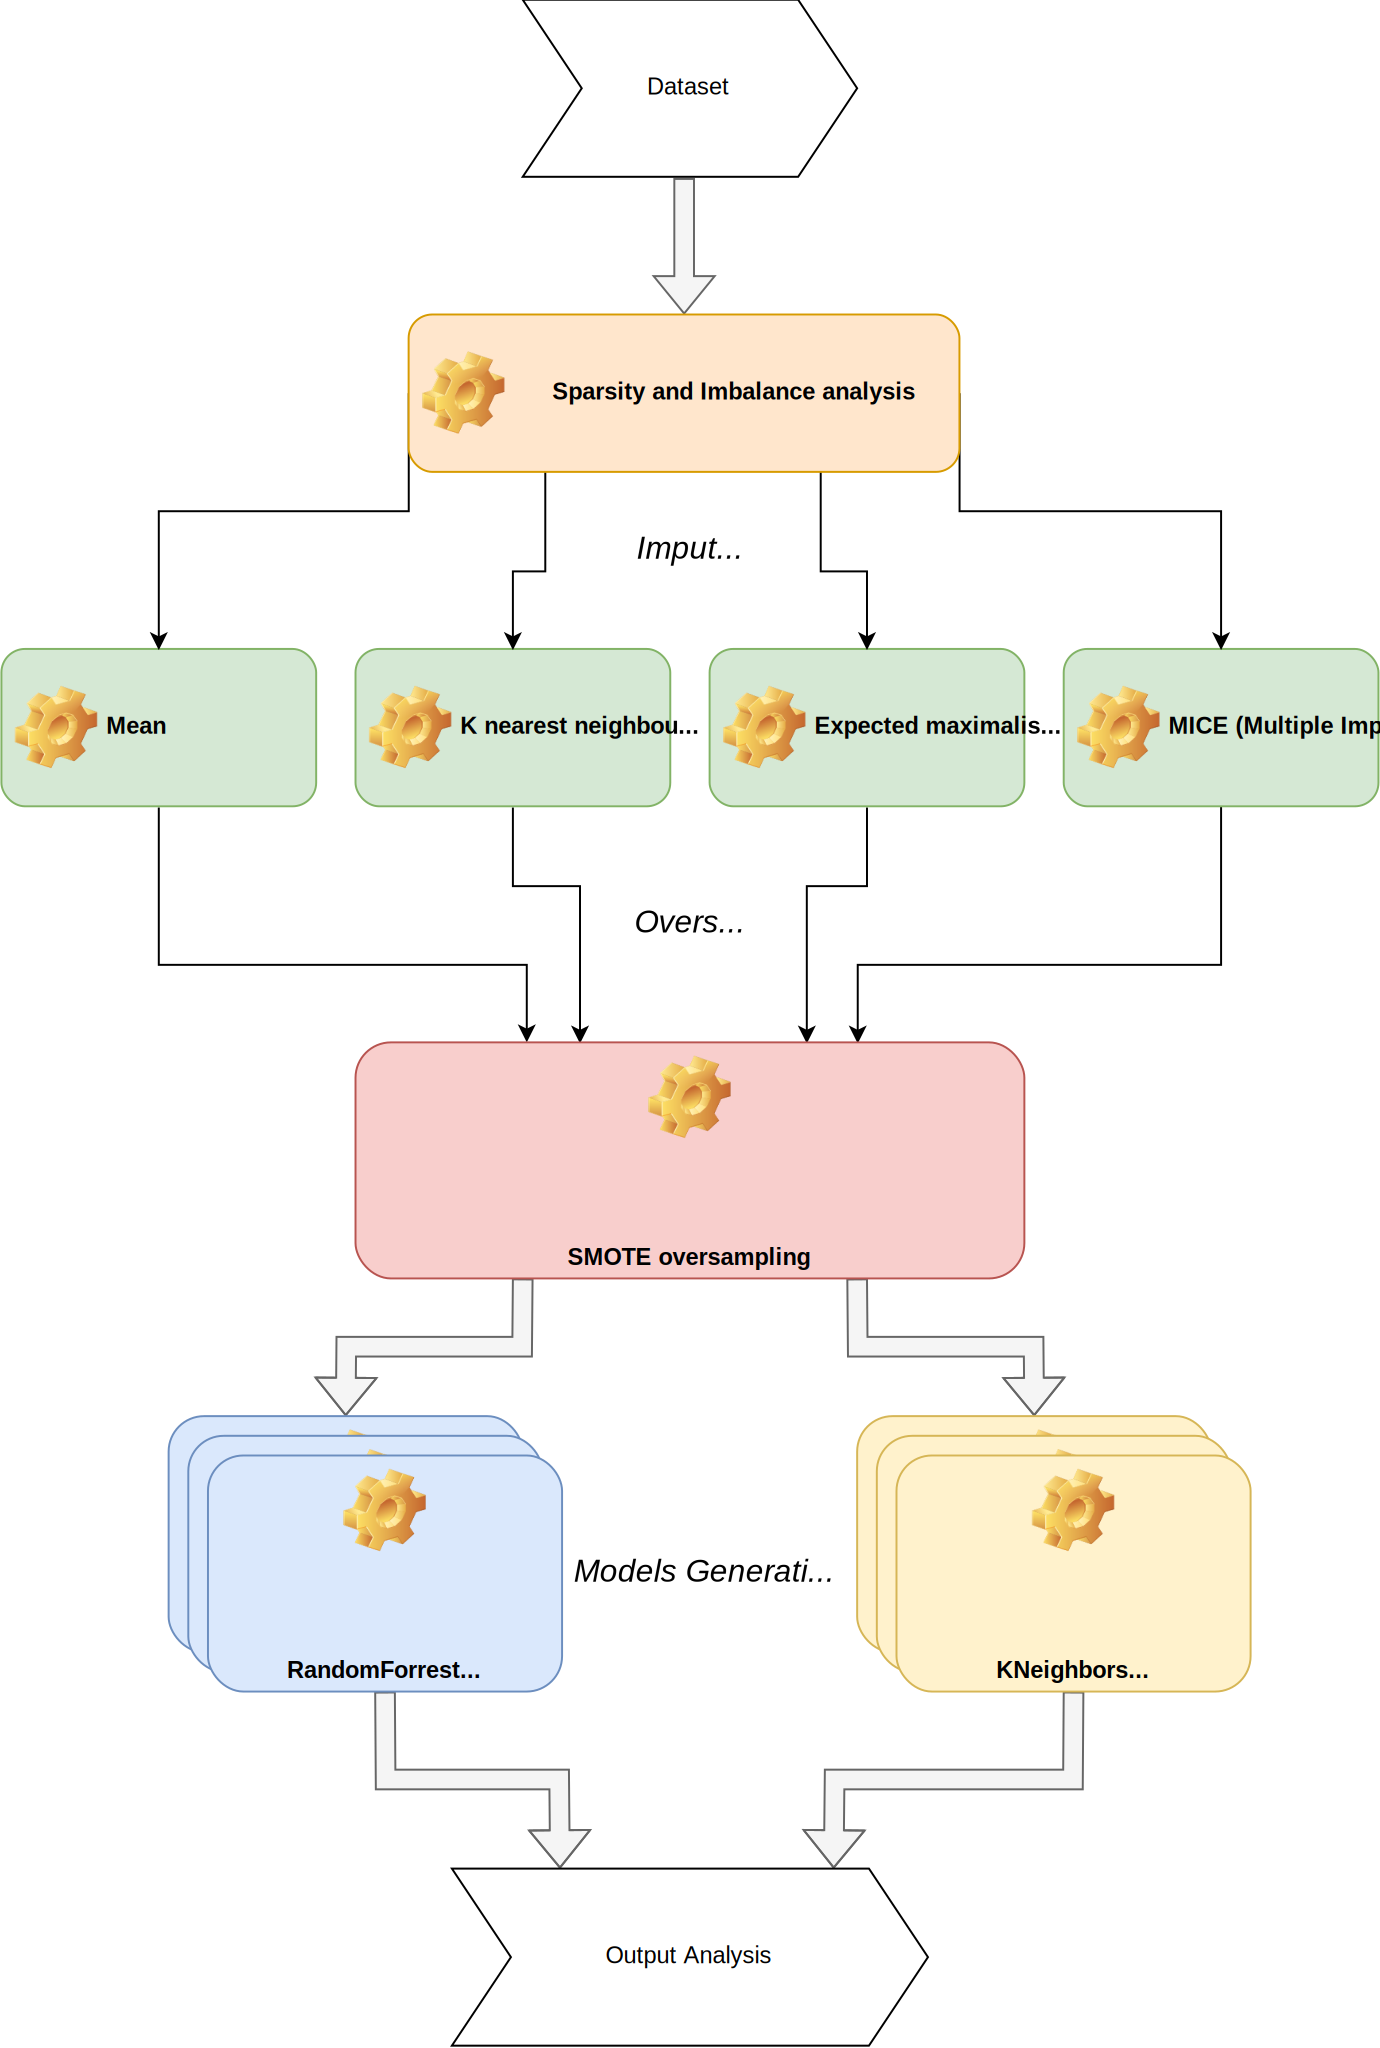
\includegraphics[width=4in]{Dataflow}
	\end{center}
\end{figure}
\section{Modele}
Zgodnie z poleceniem wykorzystaliśmy algorytmy tworzenia modeli : 
\begin{itemize}
	\item Las Losowy \textit{[RF - Random Forrest]}
	\item K Najbliższych sąsiadów \textit{[KNN - K Nearest Neighbors]}
\end{itemize}
Implementacje wymienionych algorytmów pochodzą z biblioteki \textit{sklearn}.
\subsection{Parametry Modeli}
% Paramsy i ile tych modeluf
% tabelka dla RT i KNN
\section{Wyniki Eksperymentu}    
\subsection{Wykresy}
% wykresy jak robiom dobrze imputery
% wykresy jak robiom dobrze modele 
% wykresy jak robiom dobrze modele w zależności od paramsów
\subsection{Interpretacja}
% jakiś komentarz do obrazków powyżej jeśli nie bezpośrdenio pod nimi ???
% wnioski że najlepszy np Las Losowy z tymi paramsami i imputerem Xd
\end{document}
